\doublespacing
\chapter{Background}
This chapter introduces the tree editing problem and the related algorithms. The underlying concepts of the tree editing problem are first provided, followed by a naive algorithm. Then a number of improved algorithms based on closely related dynamic programming approaches are introduced. 

\section{String Edit Distance Problem}
Before we introduce the tree edit distance problem, we first describe the string edit distance problem because the string edit distance problem can be seen as a special case of the tree edit distance problem.

First introduced by Wagner and Fischer~\cite{wagner1974string}, the string edit distance problem is to find the minimum cost to change one string$S_1$ into the other$S_2$ by a sequence of edit steps. The string edit distance problem can be solved by dynamic programming. The string edit distance $d(S_1, S_2)$ can be computed by Equation 1 where $u$ and $v$ are both the last elements or the first element of string $S_1$ and $S_2$. The cost of the three basic edit operations( substitution, deletion and insertion) are $\delta(u, v)$, $\delta(u, \varnothing)$ and $\delta(\varnothing, v)$.

\begin{definition}
(String Edit Distance)
The edit distance between strings $S_1$ and $S_2$ is the minimum cost to change $S_1$ to $S_2$ via a sequence of basic edit steps. 
\end{definition}

\section{Tree Edit Distance Problem}

The tree edit distance problem was first introduced by Tai as a generalization of the string edit distance problem~\cite{wagner1974string}. 

\begin{definition}
(Tree Edit Distance)
The edit distance between two trees $T_1$ and $T_2$ is the minimum cost to change $T_1$ to $T_2$ via a sequence of basic edit steps. 
\end{definition}

Analogous to the string edit distance problem, the basic operations are substitution with the cost $\delta(t_1, t_2)$, insertion with the cost $\delta(\varnothing, t_2)$ and deletion with the cost $\delta(t_1, \varnothing)$, where $t_1$ and $t_2$ is a node in tree $T_1$ and $T_2$ respectively. The concept of basic operations in the tree edit distance problem is similar to that in the string edit distance problem. Substitution means changing a tree node into another. Insertion first insert a node into a tree. If the inserted node is the children of a node in the tree, the children of this node become the children of the inserted node. In contrast to insertion, deletion first delete a node from a tree then the children of the deleted node become the children of the parent of the deleted node. Figure 2.1 illustrates these editing operations.

\begin{figure}
		\centering
		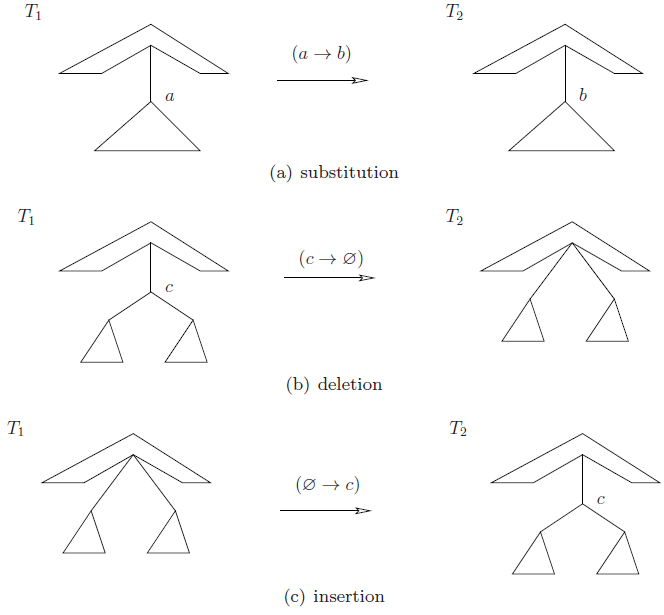
\includegraphics[width=11cm,clip]{Figures/TreeEditingOperation}
		\label{Basic tree edit operations} 
		\caption{Basic tree edit operations From ~\cite{chen2015review}. (a) substitution, (b) deletion, (c) insertion.}
\end{figure}

In this thesis, we focus on the general editing problem, which means no additional constraints are added on the order of insertions and deletions. In other words, insertions and deletions can take place in any order at any node within the tree. However, the substitution operation should satisfy the following constraints:

1. One-to-one relationship: A node in one tree can be replaced at most one node in another tree. 

2. Sibling order is preserved: For any two substitution steps($t_1[i] \to t_2[j]$) and ($t_1[i'] \to t_2[j']$), $t_1[i]$ is to the left of $t_1[i']$ if and only if $t_2[j]$ is an ancestor of $t_2[j']$.

3. Ancestor order is preserved: For any two substitution step($t_1[i] \to t_2[j]$) and ($t_1[i'] \to t_2[j']$), $t_1[i]$ is an ancestor of $t_1[i']$ if and only if $t_2[j]$ is an ancestor of $t_2[j']$.

These constraints of the preservation of sibling and ancestor order are shown in Figure 2.2.

\begin{figure}
		\centering
		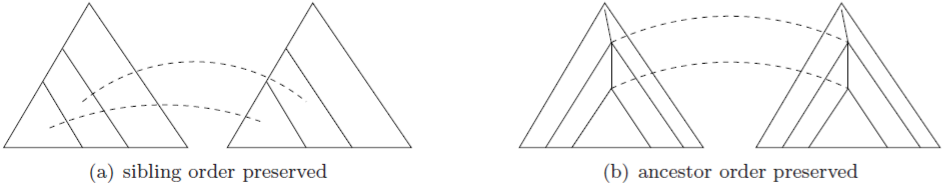
\includegraphics[width=14cm,clip]{Figures/TreeEditingOperationConstraint}
		\label{Sibling orders and ancestor orders preservation} 
		\caption{Tree editing constraints on sibling orders and ancestor orders preservation From ~\cite{chen2015review}. (a) sibling order preservation. (b) ancestor order preservation.}
\end{figure}

\section{Preliminaries}
Before we study the tree edit distance problem, it would be beneficial to define some notations, which can help analyze the algorithm clearly. 

Firstly, trees and forests should be clearly defined as they are objects in algorithms. 

\begin{definition}
(Tree and forests)
A tree is a node connected to an ordered sequence of disjoint trees. Such a sequence of tree is called a forest~\cite{dulucq2005decomposition}. 
\end{definition}

In this thesis, we only consider ordered and labeled tree. The word forest may be used for denoting forests, trees as well as a node which are reduced from a tree after a series of deletions. 

Some classical notations for trees and forests are introduced.  

\begin{notation} Let T be a tree, which is composed of a node $l$ connected to the sequence of trees $T_1, \cdots ,T_n$, T can be written as $l(T_1  \comp \cdots \comp T_n)$.
\begin{itemize}
\item $r(T)$ denotes the root of T, which is $l$ in the tree representation form of $l(T_1 \comp \cdots \comp T_n)$.
\item $T^{\comp}$ denotes the forest F after deleting r(T), that is $T_1 \comp \cdots \comp T_n$.
\item $lr(T)$ denotes the root of the leftmost tree in the forest $T^{\comp}$, that is the root of $T_1$.
\item $rr(T)$ denotes the root of the rightmost tree in the forest $T^{\comp}$, that is the root of $T_n$.
\end{itemize}
\end{notation}

\begin{notation}Let F be a forest of the form of $T_1 \comp \cdots \comp T_n$, where $T_1, \cdots ,T_n$ are trees in the forest.

\begin{itemize}
\item $\left\vert F \right\vert$ denotes the size of F, which is the number of nodes in the forest.
\item $\#leaves(F)$ denotes the number of leaves of F.
\item $depth(F)$ denotes the depth of F, that is the maximal depth of the trees in F.
\item $F(i)$, where i is a node of F, denotes the sub-tree of F rooted at i.
\item $F - i$, where i is a node of F, denotes the forest after deleting node i.
\item $lr(F)$ denotes the root of the leftmost tree in the forest $T_1 \comp \cdots \comp T_n$, that is the root of $T_1$.
\item $rr(F)$ denotes the root of the rightmost tree in the forest $T_1 \comp \cdots \comp T_n$, that is the root of $T_n$.
\end{itemize}
\end{notation}

\section{Recursive Decomposition Solution}
Before we study the recursive decomposition in the tree edit distance problem, we recall the the recursive decomposition in the string edit distance problem. The string edit distance problem can be solved by measuring the distance for all pairs of prefixes or suffixes of two strings.

The edit distance between two strings $S_1$ and $S_2$ can be computed by equation as follows:
\begin{align}
d(S_1, S_2) = min \begin{cases}
	  	d(S_1 - u , S_2) + \delta(u, \varnothing) \\ 
      	d(S_1, S_2 - v) + \delta(\varnothing, v) \\ 
    	d(S_1 - u, S_2 - v) + \delta(u, v) & \\ 
    \end{cases}
\end{align}

It is a right decomposition if and only if $u$ and $v$ are both the last element of the string $S_1$ and $S_2$. Similarly, when $u$ and $v$ are both the first element of the string $S_1$ and $S_2$, it is a left decomposition. Implementation of the string edit distance is the completion with a two-dimensional table, which gives a $\mathcal{O}(n^2)$ solution.

Analogous to the string edit distance problem, the tree edit distance can be solved in a recursive decomposition way. To compute the tree edit distance,  the roots of the trees are the first elements to decompose. The Equation 2.2 computes the tree-to-tree distance.

Let $T_1$ and $T_2$ are both trees, 
\begin{align}
d(T_1, T_2) = min \begin{cases}
	  	d(T_1 - r(T_1) , T_2) + \delta(r(T_1), \varnothing) \\ 
      	d(T_1, T_2 - r(T_2)) + \delta(\varnothing, r(T_2)) \\ 
    	d(T_1 - r(T_1), T_2 - r(T_2)) + \delta(r(T_1), r(T_2)) & \\
    \end{cases}
\end{align}

The decomposition to trees create sub-problems for forests($T_1 - r(T_1), T_2 - r(T_2)$). Similar to the Equation 2.1 for the calculation of the string edit distance, let $F_1$ and $F_2$ are both forests and $u$ and $v$ are nodes in forest $F_1$ and $F_2$ respectively, the forest-to-forest distance can be computed by equation as follows: 
\begin{align}
d(F_1, F_2) = min \begin{cases}
	  	d(F_1 - u , F_2) + \delta(u, \varnothing) \\ 
      	d(F_1, F_2 - v) + \delta(\varnothing, v) \\ 
    	d(F_1 - F(u), F_2 - F(v)) + \delta(F(u), F(v))& \\ 
    \end{cases}
\end{align}

Analogous to the string edit distance problem, the computation of forest-to-forest takes on two possible directions: left and right decomposition. Figure 2.3 illustrates the left and right decomposition.
\begin{itemize}
\item left decomposition where $u$ and $v$ are $lr(F_1)$ and $lr(F_2)$ respectively.(Figure 2.3 (a-1), (b-1), (c-1)).
\item right decomposition where $u$ and $v$ are $rr(F_1)$ and $rr(F_2)$ respectively.(Figure 2.3 (a-2), (b-2), (c-2)).
\end{itemize}

\begin{figure}
		\centering
		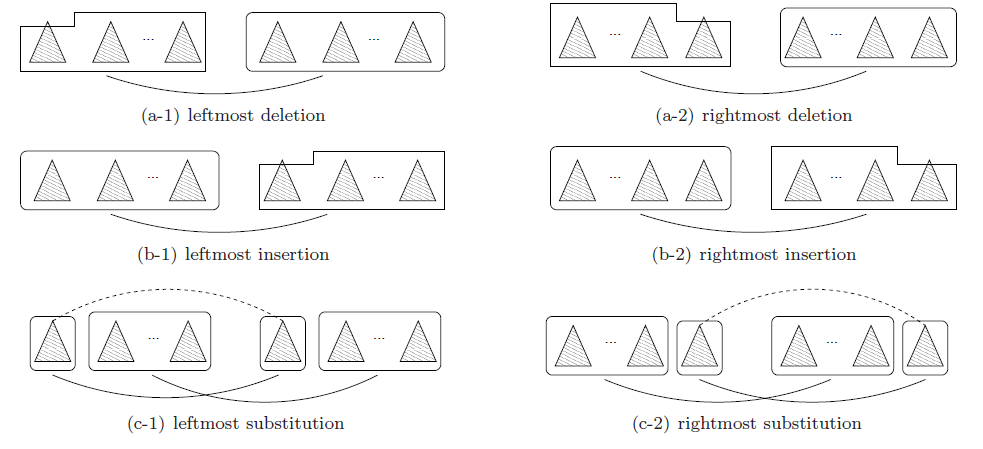
\includegraphics[width=16cm,clip]{Figures/LeftRightDecomposition}
		\label{Left and Right Recursive composition} 
		\caption{Left and Right decomposition From ~\cite{Chen2014}. (a-1) leftmost deletion. (b-1) rightmost insertion. (c-1) leftmost substitution. (a-2) rightmost deletion. (b-2) rightmost insertion. (c-2) rightmost substitution.}
\end{figure}

\section{Relevant SubForests and SubTrees}
The recursive decomposition creates relevant sub-forests recursively. 

\begin{definition}
(Relevant sub-forest)
The relevant sub-forests are the forests that appear in the recursive calls in the Equation 2.2 and 2.3. 
\end{definition}

The set of all sub-forest resulting from any decomposition from the forest F is called the full decomposition, denoted by $\mathcal{A}(F)$.

\begin{definition}
(Full decomposition)
The full decomposition of a tree is the set of all sub-forests of F obtained by recursively removing the leftmost and rightmost root nodes, $lr(F)$ and $rr(F)$, from F and the resulting sub-forests. 
\begin{equation*}
\mathcal{A}(\varnothing) = \varnothing
\end{equation*}
\begin{equation*}
\mathcal{A}(F) = \{F\} \cup \mathcal{A}(F - rr(F)) \cup \mathcal{A}(F - lr(F))
\end{equation*}
\end{definition}

Figure 2.4 illustrates the relevant sub-forests of a tree resulting from the full decomposition of a tree F.
\begin{figure}
		\centering
		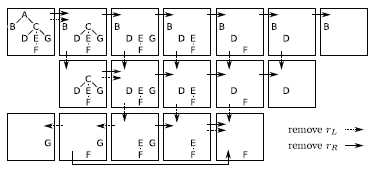
\includegraphics[width=8cm,clip]{Figures/FullDecomposition}
		\label{Relevant Sub-forests Resulting From the Full Decomposition} 
		\caption{Relevant sub-forests resulting from the full decomposition. From ~\cite{pawlik2015efficient}.}
\end{figure}

To decompose a tree, leftmost or rightmost root node can be chosen at each recursive step, resulting in the path decomposition, which is a subset of the full decomposition. Each choice of direction in each step is called a decomposition strategy. The set of decomposition strategies can be indicated by a root-leaf path.

\begin{definition}
(Root-leaf path)
The root-leaf path indicates the choice of decomposition strategy at each step in the recursive call. If the rightmost root of forest $F_1$ or $F_2$ is on the path, then $u = lr(F_1)$ and $v = lr(F_2)$ in the Equation 2.3. On the contrary, if the leftmost root of forest $F_1$ or $F_2$ is on the path, then $u = rr(F_1)$ and $v = rr(F_2)$
\end{definition}

The set of sub-forests decomposed by a root-leaf path from the forest F is called the path decomposition, denoted by $\mathcal(F)(F)$.

\begin{definition}
(Path decomposition) Path decomposition is a set of sub-forests of F obtained by recursively removing the leftmost or rightmost root nodes, $lr(F)$ and $rr(F)$, from F and the resulting sub-forests. 
\begin{equation*}
\mathcal{F}(\varnothing) = \varnothing
\end{equation*}
\begin{equation*}
\mathcal{F}(F) = \{F\} \cup \begin{cases}
	  	\mathcal{F}(F - rr(F))\\ 
      	\mathcal{F}(F - lr(F))\\ 
    \end{cases}
\end{equation*}
\end{definition}




Figure 2.5(a) is an example of relevant sub-forests that result from the leftmost path decomposition, which successively delete the rightmost root of the resulting forest. This creates 15 relevant sub-forests.Symmetrically, the rightmost path decomposition creates 11 relevant sub-forests(Figure 2.5(b)).

\begin{figure}
		\centering
		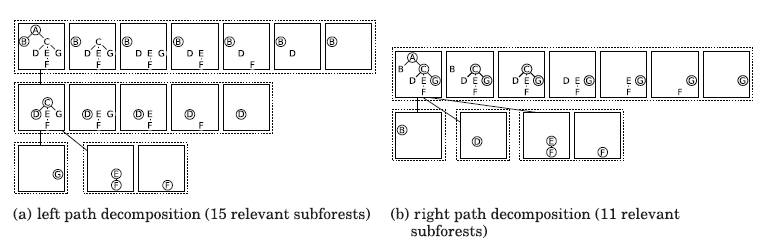
\includegraphics[width=16cm,clip]{Figures/PathDecomposition}
		\label{Relevant Sub-trees from the leftmost path decomposition and the rightmost path decomposition} 
		\caption{Relevant sub-forests. From ~\cite{pawlik2015efficient}. (a) Relevant sub-forests from the leftmost path decomposition. (b) Relevant sub-forests from the rightmost path decomposition.}
\end{figure}

\begin{definition}
(Relevant sub-trees)
The relevant sub-trees of tree T for a root-leaf path are all sub-trees that result from removing the path from T, that is, all sub-trees of T that are connected to a node of the path.  
\end{definition}

As shown in Figure 2.6, the black nodes belong to the root-leaf path and the white nodes are connected to one of the node on the path. The sub-trees rooted at the white nodes are sub-tree result from the path decomposition. 

\begin{figure}
		\centering
		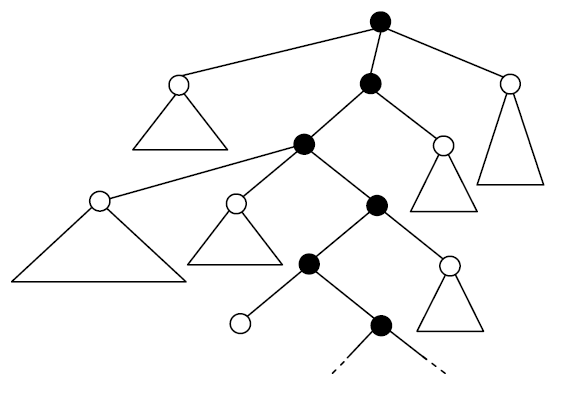
\includegraphics[width=8cm,clip]{Figures/RelevantSubtrees}
		\label{Relevant Sub-trees from the path decomposition} 
		\caption{Relevant sub-forests. From ~\cite{demaine2009optimal}.}
\end{figure}

\begin{notation}
Let T be a tree, $\gamma$ be a root-leaf path.
\begin{itemize}
\item $\Gamma(T)$ denotes the set of roots of relevant sub-trees partitioned by the path $\gamma$.
\end{itemize}

\end{notation}

So far, we have considered relevant sub-trees and sub-forests with respect to a single root-leaf path. If a root-leaf path can be defined for each of the resulting sub-trees of tree T,  the path decomposition can be recursively applied to all resulting sub-trees. This procedure is called the recursive path decomposition.
\section{Bottom-up Enumeration}
The space-efficient implementations of the tree edit distance use a bottom-up approach, which computes distance between smaller pairs of sub-trees first. In contrast to the top-down decomposition, the bottom-up enumeration order the sub-trees computation carefully to make sure all the sub problems from the Equation 2.2 and 2.3 have already been computed beforehand. 

The order of bottom-up enumeration is closely related to the top-down recursive decomposition. The top-down recursive path decomposition can be categorized into two approaches.

\begin{itemize}
\item the recursion direction is fixed to be either leftmost or rightmost,
\item the recursion direction may vary between leftmost and rightmost.
\end{itemize}

For either approach, we need an approach to enumerate the sub-problems. For the fixed direction recursion, one way to enumerate the sub problems is enumerate sub-trees as well as the sub-forests contained in each sub-tree in left-to-right or right-to-left postorder. 

\begin{itemize}
\item LR-postorder: The sub-trees as well as the sub-forests contained in each sub-trees are enumerated in left-to-right postorder.
\item RL-postorder: The sub-trees as well as the sub-forests contained in each sub-trees are enumerated in right-to-left postorder.
\end{itemize}

Figure 2.7 is an example of relevant sub-forests that result from tree T and each of its relevant sub-trees with respect to the leftmost path. The top-down view gives the recursive right decomposition while the bottom-up gives the left-to-right postorder enumeration. 

\begin{figure}
		\centering
		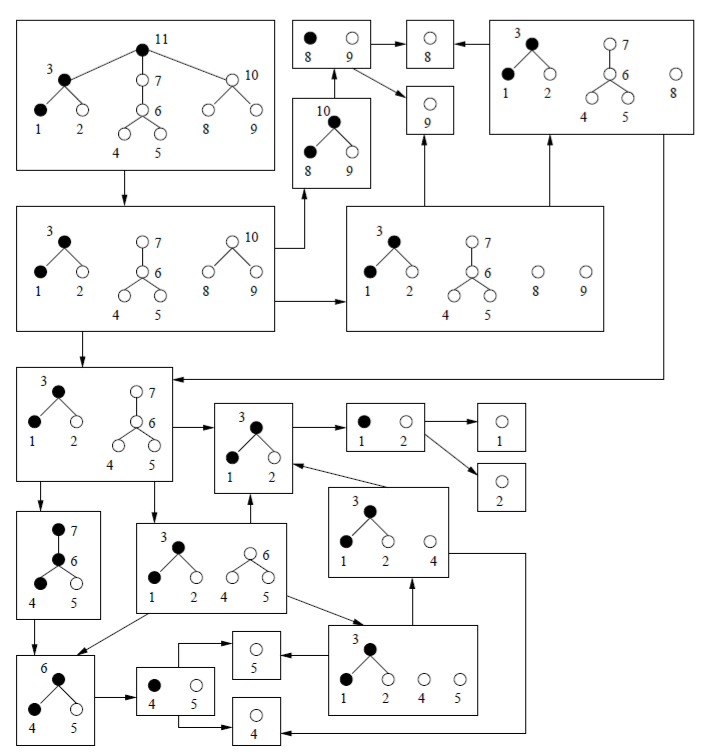
\includegraphics[width=12cm,clip]{Figures/LeftToRightEnumeration}
		\label{Relevant Sub-forests that Result From the Leftmost Path Decomposition} 
		\caption{Relevant sub-forests that result from the leftmost path decomposition. From ~\cite{Chen2014}.}
\end{figure}

To enumerate the full decomposition, two approaches can be used, which is suffix-prefix and prefix-suffix postorder enumeration. In prefix-suffix postorder enumeration leftmost root is fixed then enumerate each nodes in the sub-tree, whereas rightmost root is fixed then enumerate each nodes in the sub-tree in suffix-prefix postorder. 

\begin{itemize}
\item prefix-suffix postorder: Enumerate the rightmost root in left-to-right postorder then enumerate the leftmost root in the tree. 
\item suffix-prefix postorder: Enumerate the leftmost root in right-to-left postorder then enumerate the rightmost root in the tree.
\end{itemize}

Figure 2.8 and Figure 2.9 is the example of prefix-suffix order enumeration and suffix-prefix order enumeration respectively. In Figure 2.10, sub-forests having the same rightmost root are in contiguous boxes while sub-forests having the same leftmost root are in contiguous boxes.

\begin{figure}
		\centering
		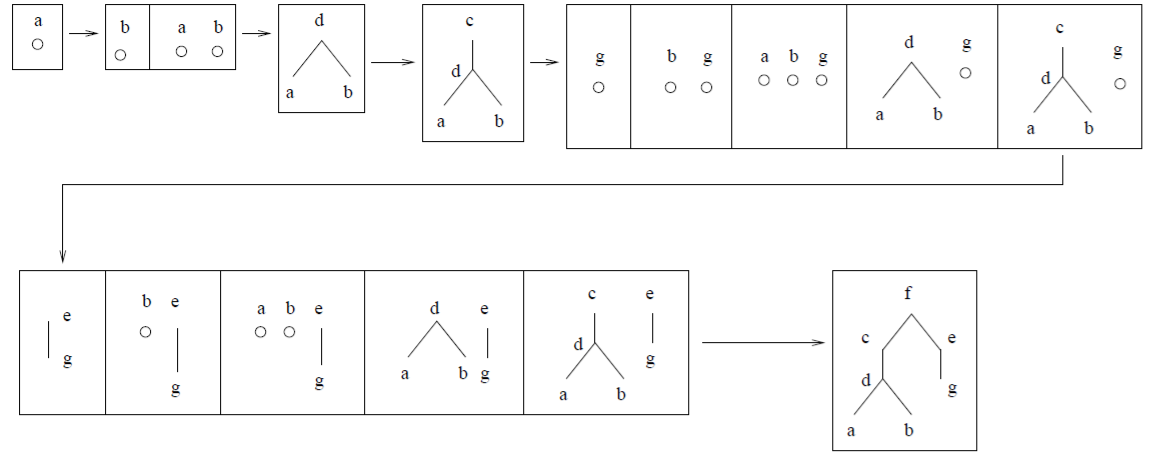
\includegraphics[width=12cm,clip]{Figures/PrefixSuffixPostorder}
		\label{Prefix-suffix Postorder Enumeration} 
		\caption{An example of enumerating subforests in prefix-suffix postorder. From ~\cite{Chen2014}.}
\end{figure}

\begin{figure}
		\centering
		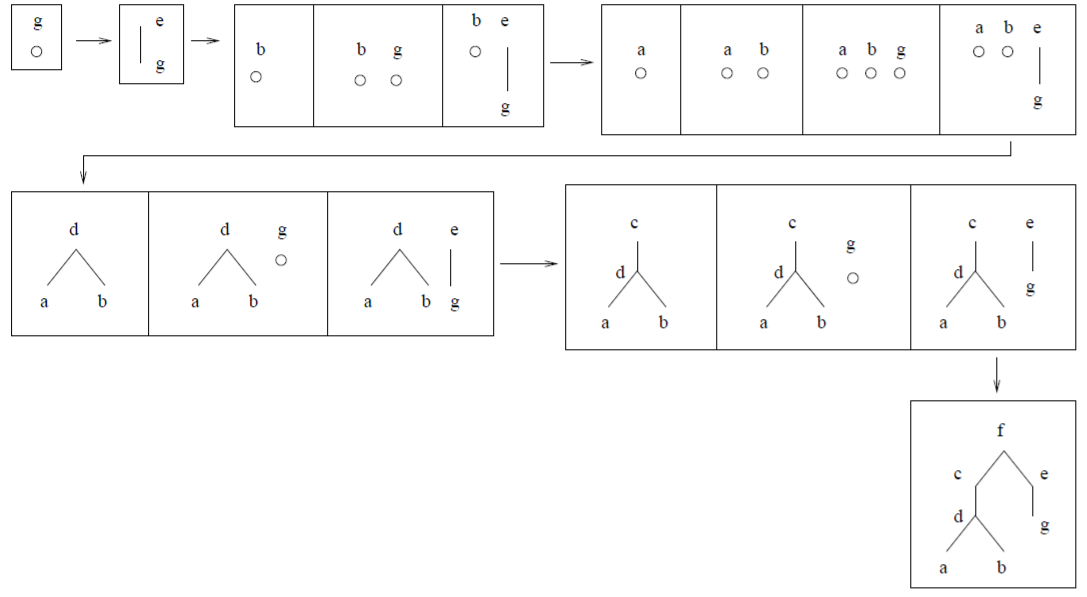
\includegraphics[width=12cm,clip]{Figures/SuffixPrefixPostorder}
		\label{Suffix-prefix Postorder Enumeration} 
		\caption{An example of enumerating subforests in suffix-prefix postorder. From ~\cite{Chen2014}.}
\end{figure}

\section{A Simple Algorithm}
In this section, we provide a simple algorithm to compute the tree edit distance, which runs in $\mathcal{O}(m^{2}n^{2})$, where $m$ and $n$ are the size of tree. To compute the tree edit distance between two pairs, we need to calculate the distance of all sub-forests pairs, which are enumerate in prefix-suffix or suffix-prefix postorder. 

\begin{lemma} The full decomposition takes $\mathcal{O}(\left\vert T \right\vert ^ {2})$ steps, where $\left\vert T \right\vert$ is the size of the tree.
\end{lemma} 
\begin{proof}
We consider the prefix-suffix postorder only as the suffix-prefix postorder is symmetrical. 
Let $f_{i}$ be the number of sub-forests with distinct leftmost roots which contain $t_i$ as the rightmost root. As menetioned in section 2.6, to enumerate the full decomposition in prefix-suffix postorder, first fix the rightmost root then enumerate the leftmost root in the tree in right-to-left postorder. Summing over all nodes to enumerate, we have $\sum_{i=1}^{\left\vert T \right\vert} \leq \sum_{i=1}^{\left\vert T \right\vert} \left\vert T \right\vert = \mathcal{O}(\left\vert T \right\vert^{2})$
\end{proof}

By enumerating all pairs of sub-forests between two trees, the tree edit distance can be calculated.  Here is a simple algorithm runs in $\mathcal{O}(m^2n^2)$ time using $\mathcal{O}(m^2n^2)$ space.

\IncMargin{1em}
\begin{algorithm}
  \caption{Compute tree edit distance by enumerating all pairs in $\mathcal{O}(m^2n^2)$ time.}
  \SetKwInOut{Input}{inputs}
  \SetKwInOut{Output}{output}
  \SetKwData{TreeA}{$T_1$}
  \SetKwData{TreeB}{$T_2$}
  \SetKwData{SizeOfTreeA}{$\left\vert T_1 \right\vert$}
  \SetKwData{SizeOfTreeB}{$\left\vert T_2 \right\vert$}
  \SetKwFunction{POSTORDER}{POSTORDER}{}{}

  \Input{ (\TreeA , \TreeB), with \SizeOfTreeA = $m$ and \SizeOfTreeB = $n$ }
  \Output{$d(T_1[i], T_2[j])$ for $1 \leq i \leq m$ and $1 \leq j \leq n$}
    $L_1 \gets \POSTORDER(T_1)$\;
    $L_2 \gets \POSTORDER(T_2)$\;
    \For{$i=1$ \KwTo $\left\vert L_1 \right\vert$} {
		\For{$j=1$ \KwTo $\left\vert L_2 \right\vert$} {
			compute $d(L_1[i], L_2[j])$ as in Equation 2.3
		}    
    }
    $d(T_1[i], T_2[j]) \gets d(L_1[\left\vert L_1 \right\vert][\left\vert L_2 \right\vert])$\;
    \KwRet{$d(T_1[i], T_2[j])$}\;
\end{algorithm}
\DecMargin{1em}

\begin{lemma}
The upper bound of the post-order enumeration method for tree edit distance problem is $\mathcal{O}(m^2n^2)$, where $m$ and $n$ are the size of two trees.
\end{lemma}
\begin{proof}
From lemma 2.7.1, the upper bound(full decomposition with no assumption on the strategy) of the number of relevant sub-forests for one tree of size $n$ is $\mathcal{O}(n^2)$. Therefore, the upper bound of the relevant sub-forests pairs of trees of sizes $m$ and $n$ respectively is $\mathcal{O}(m^2n^2)$. This concludes the proof.
\end{proof}

\section{Improved Algorithmic Path Strategies}
Leftmost or rightmost root node is chosen at each recursive step, resulting in the path decomposition, which is the subset of the full decomposition. We use a root-leaf path to indicate the set of decomposition strategies.

Different path decomposition creates different number of relevant sub-forests. Figure 2.10 and Figure 2.11 is an example of different sub-forests that result from different path decomposition strategies. In Figure 2.10, the path is rightmost path, and in Figure 2.11, the path is leftmost path. This gives respectively 7 and 9 sub-forests. Therefore, to make further improvement we look for ways to take advantage of the overlap among sub-forests that are contained in the same sub-tree, and the overlap of sub-trees as well. 

\begin{figure}
		\centering
		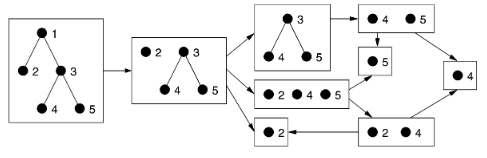
\includegraphics[width=12cm,clip]{Figures/LeftmostPathDecomposition}
		\label{Relevant Sub-forests that Result From the Leftmost Path Decomposition} 
		\caption{Relevant sub-forests that result from the leftmost path decomposition. From ~\cite{dulucq2005decomposition}.}
\end{figure}

\begin{figure}
		\centering
		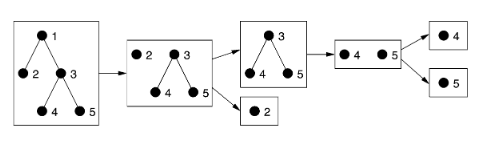
\includegraphics[width=12cm,clip]{Figures/RightmostPathDecomposition}
		\label{Relevant Sub-forests that Result From the Rightmost Path Decomposition} 
		\caption{Relevant sub-forests that result from the rightmost path decomposition. From ~\cite{dulucq2005decomposition}.}
\end{figure}

The current state-of-the art path strategies are leftmost(rightmost) paths on both tree, heavy paths on one tree as well as heavy paths on both trees.

\section{Zhang and Shasha's Algorithm}

Zhang and Shasha's algorithm~\cite{zhang1989simple} fixes the direction in each recursion, say right decomposition. The situation for the recursive left decomposition is symmetrical to that for the recursive right decomposition. 

\begin{figure}
		\centering
		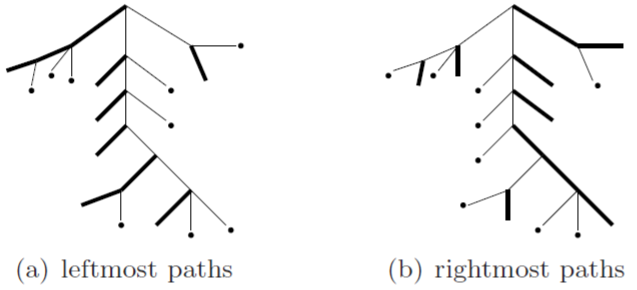
\includegraphics[width=12cm,clip]{Figures/LeftmostPathandRightmostPath}
		\label{Leftmost Paths and Rightmost Paths} 
		\caption{Leftmost paths and rightmost paths in a tree and its resulting sub-trees From ~\cite{Chen2014}.}
\end{figure}

Full decomposition is not needed in the Zhang and Shasha's algorithm since the direction to decompose is fixed. This means that only the path decomposition to the whole tree and its resulting sub-trees is needed instead of the full decomposition. This means that the enumeration of the Zhang and Shasha's algorithm will be in LR-postorder while the symmetrical rightmost paths algorithm used RL-postorder enumeration. See Figure 2.12(a) as an example of the leftmost paths applied the whole tree and its resulting sub-trees and Figure 2.12(b) is the example of rightmost paths.

Taking the advantage of the overlap among sub-trees, all sub-trees sharing the same leftmost leaf can be handled together. In other words, a set of sub-tress along the leftmost path can be handled together with the LR-postorder enumeration to avoid redundant computation.

The root of each relevant sub-trees resulted from the leftmost paths is refereed to as an "LR-keyroot", which is defined as follows.

\begin{definition}
(LR-keyroots). An LR-keyroot is either the root of T or has a left sibling.
\end{definition}

The procedure of the Zhang and Shasha's algorithm as follows. First we identify all LR-keyroots and sort them in LR-postorder. Then enumerate each pairs of relevant sub-trees in order and calculate the distance between them. 

\IncMargin{1em}
\begin{algorithm}
  \caption{Zhang and Shasha's Algorithm}
  \SetKwInOut{Input}{inputs}
  \SetKwInOut{Output}{output}
  \SetKwData{TreeA}{$T_1$}
  \SetKwData{TreeB}{$T_2$}
  \SetKwData{SizeOfTreeA}{$\left\vert T_1 \right\vert$}
  \SetKwData{SizeOfTreeB}{$\left\vert T_2 \right\vert$}
  \SetKwFunction{POSTORDER}{LR\_KEYROOT\_POSTORDER}{}{}
  \SetKwFunction{TREEDISTANCE}{TREE\_TREE\_DISTANCE}{}{}

  \Input{ (\TreeA , \TreeB), with \SizeOfTreeA = $m$ and \SizeOfTreeB = $n$ }
  \Output{$d(T_1[i], T_2[j])$ for $1 \leq i \leq m$ and $1 \leq j \leq n$}
    $L_1 \gets \POSTORDER(T_1)$\;
    $L_2 \gets \POSTORDER(T_2)$\;
    \For{$i=1$ \KwTo $\left\vert L_1 \right\vert$} {
		\For{$j=1$ \KwTo $\left\vert L_2 \right\vert$} {
			$\TREEDISTANCE(T_1(L_1[i]), T_2(L_2[j]))$
		}    
    }
    $d(T_1[i], T_2[j]) \gets d(L_1[\left\vert L_1 \right\vert][\left\vert L_2 \right\vert])$\;
    \KwRet{$d(T_1[i], T_2[j])$}\;
\end{algorithm}
\DecMargin{1em}

In function TREE\_TREE\_DISTANCE in Algorithm 2, the leftmost root is fixed and the rightmost roots are enumerated to construct relevant sub-forests. The enumeration algorithm is shown in algorithm 3.

\IncMargin{1em}
\begin{algorithm}
  \caption{TREE\_TREE\_DISTANCE}
  \SetKwInOut{Input}{inputs}
  \SetKwInOut{Output}{output}
  \SetKwData{TreeA}{$T_1(a)$}
  \SetKwData{TreeB}{$T_2(b)$}
  \SetKwData{RA}{$a$}
  \SetKwData{RB}{$b$}
  \SetKwFunction{POSTORDER}{LR\_POSTORDER}{}{}

  \Input{ (\TreeA , \TreeB)}
  \Output{$d(T_1(a), T_2(b))$}
    $L_1 \gets \POSTORDER(T_1(a))$\;
    $L_2 \gets \POSTORDER(T_2(b))$\;
    \For{$i=1$ \KwTo $\left\vert L_1 \right\vert$} {
		\For{$j=1$ \KwTo $\left\vert L_2 \right\vert$} {
			$rr\_F_1 \gets L_1[i]$\;
			$rr\_F_2 \gets L_2[j]$\;
			
			\uIf{$rr\_F_1 == lr(T_1(a)) \land rr\_F_2 == lr(T_2(b))$ } {
				compute $d(T_1(rr\_F_1),  T_2(rr\_F_2))$ as in Equation 2.2\;
			}
			\uElse {
				compute $d((lr(T_1(a), rr\_F_1), (lr(T_2(b)), rr\_F_2))$ as in Equation 2.3\;		
			}		
		}    
    }
    \KwRet{$d(T_1(a), T_2(b))$}\;
\end{algorithm}
\DecMargin{1em} 

\begin{lemma}
The time complexity of Zhang and Shasha's algorithm is $\mathcal{O}(mn \times min\{depth(T_1), \#leaves(T_1)\} \times min\{depth(T_2), \#leaves(T_2)\})$
\end{lemma}
\begin{proof}
Each sub problems can be solved in constant time. Thus, the time complexity can be counted by the number of sub problems. According to the enumeration scheme from algorithm 3, the number can be counted by the occurring of each node representing as the rightmost root in relevant sub-forests. The maximal times a node representing the rightmost root of relevant sub-forests can be estimated by the maximal number of non-leaf LR-keyroots that a path in the tree may contain. Firstly, since the number of LR-keyroots on any path is bounded by the depth of the path, the number of sub problems is bounded by $\#depth(T)$. Secondly, the number of sub-trees can not exceed the number of leaves as each relevant sub-trees in the Zhang and Shasha's algorithm have distinct leftmost leaves. Therefore, the number of relevant sub-trees decomposed by a leftmost path is bounded by $depth(T)$ or $\#leaves(T)$, whichever is smaller. Therefore the number of sub-forests in either tree is $\left\vert T \right\vert \times min\{depth(T), \#leaves(T)\}$  
\end{proof}
\begin{lemma}
The tree edit distance problem can be solved in $\mathcal{O}(mn)$ space, where $m=\left\vert T_1 \right\vert$ and $n=\left\vert T_2 \right\vert$
\end{lemma}
\begin{proof}
Dynamic programming method is used to implement, which fills out two $m \times n$ tables. One permanent matrix stores the tree-tree distance and the other temporary matrix stores the forest-forest distance. The temporary forest-forest distance matrix can be overwritten when the computation moves from one pair of relevant sub-trees to another pair. Besides, the permanent tree-tree distance matrix are fetched for use in computing forest-forest distances.
\end{proof}
\section{Klein's Algorithm}
Zhang and Shasha's algorithm improves the time complexity by taking the advantage of the overlap of  sub-forests with the same leftmost root. However, the running time can be improved in some trees as it is dependent on shapes of trees. Kelvin~\cite{klein1998computing} explored and designed a new decomposition strategy based on a type of path called "heavy path". Zhang and Shasha's algorithm ignores shapes of trees and fixes the direction in each decomposition steps while the direction may change in each steps according to different tree shapes. 

Heavy child and heavy paths was first introduced by Harel and Tarjan\cite{harel1984fast}. The definition is as follows.

\begin{definition}
(Heavy Child)
For any node t in Tree T, the heavy child is the root of the largest sub-trees among the sibling sub-trees, denoted by $heavy(t)$.
\end{definition}

\begin{definition}
(Heavy Path)
The descending path of Tree T from root to leaf consists of the sequence of nodes $r, heavy(r), heavy(heavy(r)) \cdots$ is called the heavy path, denoted by $P(T)$
\end{definition}

Figure 2.13 is an example of heavy paths. In the left picture, a tree's heavy path is indicated in bold. The figure on the right depicts heavy paths applied to the whole tree and its relevant sub-trees.

\begin{figure}
		\centering
		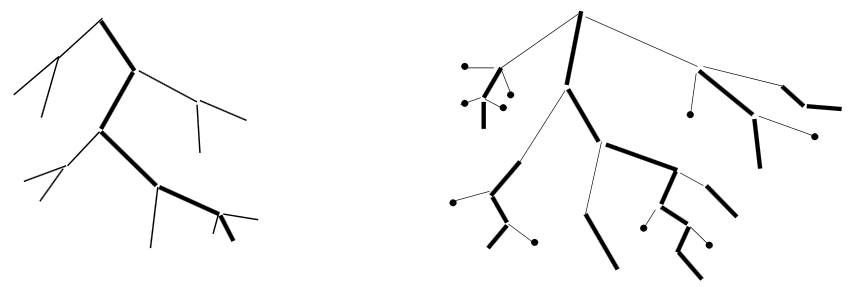
\includegraphics[width=12cm,clip]{Figures/HeavyPaths}
		\label{Heavy Paths} 
		\caption{Heavy Paths to a tree and its relevant sub-trees From ~\cite{klein1998computing}.}
\end{figure}

Let $F$ be a forest denoted as $l(f) \comp t$, where $l(f)$ is the leftmost tree in the forest, $t$ be the rest of the forest and $F'$ be another forest to compare. In Klein's algorithm, the procedure of the decomposition using the heavy path of the tree is as follows:

\begin{enumerate}
\item if $l$ belongs to the heavy path, apply right decomposition, otherwise apply left decomposition
\item apply this scheme recursively to all relevant sub-forests of $l(f) \comp t$
\end{enumerate}

Figure 2.14 illustrates the this procedure. For each step, the nodes on the heavy path are indicated by circles. 

\begin{figure}
		\centering
		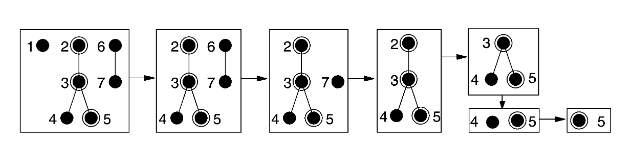
\includegraphics[width=12cm,clip]{Figures/KleinAlgorithmExample}
		\label{Example of Decomposition for Klein's Algorithm} 
		\caption{Example of decomposition for Klein's algorithm From ~\cite{klein1998computing}.}
\end{figure}

Symmetrical to Klein's decomposition, right decomposition can be first applied to relevant sub-forests then left decomposition. Let $F$ be a forest denoted as $l(f) \comp t$, where $l(f)$ is the leftmost tree in the forest, $t$ be the rest of the forest and $F'$ be another forest to compare, the procedure is shown as follows:

\begin{enumerate}
\item if $l$ belongs to the heavy path, apply left decomposition, otherwise apply right decomposition
\item apply this scheme recursively to all relevant sub-forests of $l(f) \comp t$
\end{enumerate} 

Two ways of top-down decomposition give two ways of bottom-up enumeration, referred as  "H-postorder". Nodes on the right side of the heavy child can first be enumerated in left-to-right postorder then nodes on the left side are enumerated in right-to-left postorder. Alternatively, the second version is symmetrical to the first one, i.e., right-to-left postorder then left-to-right postorder intermittently. Figure 2.15 is an example of H-postorder enumeration in Klein's algorithm.

\begin{figure}
		\centering
		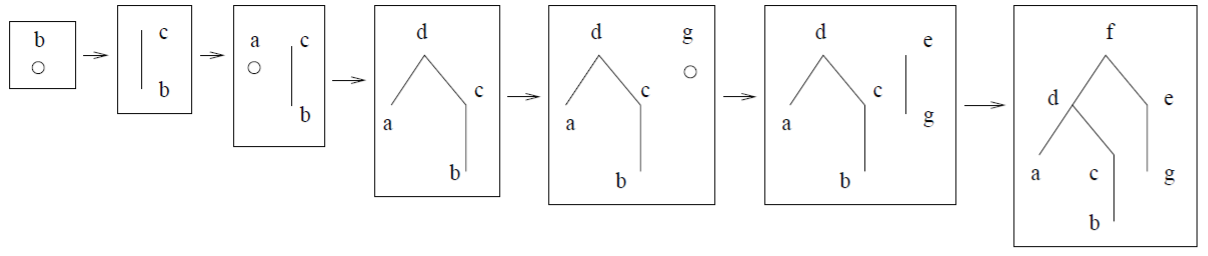
\includegraphics[width=12cm,clip]{Figures/HPostoderEnumeration}
		\label{Example of Enumerating Sub-forests in H-postorder} 
		\caption{Example of enumerating sub-forests in H-postorder From ~\cite{chen2015review}.}
\end{figure}

As listed in Algorithm 4, the keyroots in the larger tree are sorted in H-postorder. On the other hand, the full decomposition of the smaller tree is sorted in prefix-suffix or suffix-prefix postorder. Then compute each relevant sub-trees of the larger tree with respect to each relevant sub-forests of the smaller tree. 

\IncMargin{1em}
\begin{algorithm}
  \caption{Klein's Algorithm}
  \SetKwInOut{Input}{inputs}
  \SetKwInOut{Output}{output}
  \SetKwData{TreeA}{$T_1$}
  \SetKwData{TreeB}{$T_2$}
  \SetKwData{SizeOfTreeA}{$\left\vert T_1 \right\vert$}
  \SetKwData{SizeOfTreeB}{$\left\vert T_2 \right\vert$}
  \SetKwFunction{HPOSTORDER}{H\_KEYROOT\_POSTORDER}{}{}
  \SetKwFunction{FPOSTORDER}{PREFIX\_SUFFIX\_POSTORDER}{}{}
  \SetKwFunction{TREEDISTANCE}{TREE\_TREE\_DISTANCE}{}{}

  \Input{ (\TreeA , \TreeB), with \SizeOfTreeA = $m$, \SizeOfTreeB = $n$ and $m \leq n$}
  \Output{$d(T_1[i], T_2[j])$ for $1 \leq i \leq m$ and $1 \leq j \leq n$}
    $L_1 \gets \FPOSTORDER(T_1)$\;
    $L_2 \gets \HPOSTORDER(T_2)$\;
    \For{$i=1$ \KwTo $\left\vert L_1 \right\vert$} {
		\For{$j=1$ \KwTo $\left\vert L_2 \right\vert$} {
			compute $d(L_1[i], L_2[j])$ as in Equation 2.3
		}    
    }
    $d(T_1[i], T_2[j]) \gets d(L_1[\left\vert L_1 \right\vert][\left\vert L_2 \right\vert])$\;
    \KwRet{$d(T_1[i], T_2[j])$}\;
\end{algorithm}
\DecMargin{1em}
\begin{lemma}
Let $h_1, h_2, \cdots h_k$ be any nodes on the same heavy path he same path where $h_i$ is an ancestor of $h_j$ if $i < j$. Then, $\left\vert T(h_j) \right\vert \leq \left\vert T(h_i) \right\vert / 2$ if $j=i+1$
\end{lemma}
\begin{proof}
By definition, heavy child is the root of the largest sub-trees among the sibling sub-trees. Then, $\left\vert T(h_j) \right\vert \leq \left\vert T(h_i) \right\vert / 2$ is always true. Otherwise, it is a contradiction to the fact that $h_j$ is a heavy child.
\end{proof}

\begin{lemma}
The time complexity of Klein's algorithm is $\mathcal{O}(m^2n \log n)$, where $\left\vert T_1 \right\vert = m$, $\left\vert T_2 \right\vert = n$ and $m \leq n$.
\end{lemma}
\begin{proof}
Each sub problems can be solved in constant time. Thus, the time complexity can be counted by the number of sub problems. According to the enumeration scheme from algorithm 3, the number can be counted by the occurring of each node representing as the rightmost root in relevant sub-forests. The maximal times a node representing the rightmost root of relevant sub-forests can be estimated by the maximal number of non-leaf keyroots that a path in the tree may contain. From Lemma 2.10.1, for each nodes in the heavy path that is being visited, the corresponding subtree size is reduced by at least a factor of 2 with respect to its parent. In other word, it takes at most $log_2(\left\vert T \right\vert)$ steps from the root to path. That is to say, the number of sub-forests of the larger tree is bounded by $n \times log n$

Since the direction in each steps is not fixed, the full decomposition rather than the path decomposition of the smaller is needed to be considered, which creates at most $m^2$ relevant sub-forests.

To sum up, the number of pair of relevant sub-forests is $m^2n \log n$, which concludes the proof.
\end{proof}
\begin{lemma}
The space complexity of Klein's algorithm is $\mathcal{O}(mn)$, where $\left\vert T_1 \right\vert = m$, $\left\vert T_2 \right\vert = n$ and $m \leq n$. 
\end{lemma}
\begin{proof}
We use one temporary matrix of the size $m \times n$ and one permanent matrix of the size $m^2$ to store the intermediate result. The permanent matrix stores the tree-tree distance and the temporary one stores the distance between between a specific sub-tree in the larger tree and each relevant sub-forests in the full decomposition of the smaller tree. The temporary matrix can be rewritten when a new sub-tree is enumerated. Additionally, the results in the permanent tree-tree distance matrix are fetched for use in computing forest-forest distances.
\end{proof}

\section{Demaine's Algorithm}
Klein algorithm reduces the upper bound on the number of relevant sub-forests required from $\mathcal{O}(min\{depth(T), \#leaves(T)\})$ to $\mathcal{O}(\log \left\vert T \right\vert)$ for one tree. However, the cost to this strategy is having to consider all sub-forests(full decomposition) not partial sub-forests(path decomposition) in the other tree. Demaine~\cite{demaine2009optimal} improved this strategy by a way that applies the heavy path decomposition on both trees. 

Let $T_1$ and $T_2$ be two trees, assuming that $\left\vert T_1 \right\vert \leq \left\vert T_2 \right\vert$, Demaine's algorithm works as follows:

\begin{enumerate}
\item If $\left\vert T_1 \right\vert > \left\vert T_2 \right\vert$, compute $d(T_2, T_1)$
\item Recursively, compute $d(T_1, T_2(k))$ with k being the root of relevant sub-trees.
\item Compute $d(T_1, T_2)$ by enumerating full decomposition of $T_1$ in prefix-suffix or suffix-prefix postorder, and path decomposition of $T_2$ in H-postorder.
\end{enumerate}
\begin{lemma}
Let $T_1$ and $T_2$ be two trees, $R(T_1, T_2)$ be the number of relevant sub-forests pairs encountered by the algorithm, we have
\begin{equation*}
R(T_1, T_2) \leq 4(\left\vert T_1 \right\vert \left\vert T_2 \right\vert)^{\frac{3}{2}}
\end{equation*}
\end{lemma}
\begin{proof}
This can be proved by induction on $\left\vert T_1 \right\vert + \left\vert T_2 \right\vert$.

Basis: if $\left\vert T_1 \right\vert + \left\vert T_2 \right\vert = 0$, then both trees are empty and $R(T_1, T_2) = 0$ always holds.

Induction: if $\left\vert T_1 \right\vert + \left\vert T_2 \right\vert > 0$, for the case $\left\vert T_1 \right\vert \geq \left\vert T_2 \right\vert$, we have established
\begin{equation*}
R(T_1, T_2) \leq \left\vert T_2 \right\vert^2\left\vert T_1 \right\vert + \sum_{v \in \Gamma(T_1)}R(T_1(v), T_2)
\end{equation*} 
We consider the first case only for the other case when $\left\vert T_1 \right\vert < \left\vert T_2 \right\vert$ is symmetric.
Hence, by the induction hypothesis,
\begin{align}
R(T_1, T_2) &\leq \left\vert T_2 \right\vert^2\left\vert T_1 \right\vert + \sum_{v \in \Gamma(T_1)}4(\left\vert T_1(v) \right\vert \left\vert T_2 \right\vert)^(\frac{3}{2})\\
&= \left\vert T_2 \right\vert^2 \left\vert T_1 \right\vert + 4\left\vert T_2 \right\vert^{\frac{3}{2}}\sum_{v \in \Gamma(T_1)}\left\vert T_1(v) \right\vert^{\frac{3}{2}}
\end{align}
We observed that any tree $T$ has the following two properties:
\begin{itemize}
\item $\sum_{v \in \Gamma(T)}\left\vert T(v) \right\vert \leq \left\vert T \right\vert$. Because either relevant sub-trees in tree $T$ is disjoint.
\item $\left\vert T(v) \right\vert \leq \frac{\left\vert T \right\vert}{2}$ for  any sub-trees in the set $\Gamma(T)$.
\end{itemize}
Applying these two inequalities to Equation 2.5, we have
\begin{align*}
R(T_1, T_2)
&\leq \left\vert T_2 \right\vert^2 \left\vert T_1 \right\vert + 4\left\vert T_2\right\vert^{\frac{3}{2}} \sum_{v \in \Gamma(T_1)}max_{v \in \Gamma(T_1)} \sqrt{\left\vert T_1(v) \right\vert}\\
&\leq \left\vert T_2 \right\vert^2 \left\vert T_1 \right\vert + 4\left\vert T_2 \right\vert^{\frac{3}{2}}\left\vert T_1 \right\vert \sqrt{\frac{\left\vert T_1 \right\vert}{2}}\\
&=\left\vert T_2 \right\vert^2\left\vert T_1 \right\vert + \sqrt{8}(\left\vert T_1 \right\vert \left\vert T_2 \right\vert)^{\frac{3}{2}}\\
&\leq 4(\left\vert T_1 \right\vert\left\vert T_2 \right\vert)^{\frac{3}{2}}
\end{align*}
\end{proof}

\begin{lemma}
The time complexity of Demaine's algorithm is $\mathcal{O}(m^2n(1+\log{\frac{n}{m}}))$, where $\left\vert T_1 \right\vert =m$, $\left\vert T_2 \right\vert = n$, and $m \leq n$.
\end{lemma}
\begin{proof}
To analyze the time complexity, we count the total number of sub-problems. Step (2) produces recursive calls for each pairs of relevant sub-trees while every new relevant sub-problems is created in step (3). 
In step (2), the algorithm computes distance between tree pairs $(T_1(v), T_2)$ for all $v \in $. Hence, the number of sub-problems encountered in this step (2) is $\sum_{v \in \Gamma{T_1}}R(T_1(v), T_2)$. 
Therefore, we define set $A, B \subset T_1$ as follows:
\begin{itemize}
\item $A = \{a \in light(T_1) \cap \left\vert T_1(a) \right\vert \geq m \}$
\item $B = \{b \in T_1 - A\}$
\end{itemize}
For each $v \in \Gamma(T_1)$, notice that $v$ is either in A or B. It is in A if $\left\vert T_1(v) \right\vert \geq m$, and in B otherwise. If $v \in A$, all sub-problems arising from the computation of $(T_1(u), T_2)$ for $u \in \Gamma(T_1(v))$. If $v \in B$, the sub-problems is from the recursive call in step (2).For each nodes $a$ in set A, the number of sub-problems produced in step(3) is $\left\vert T_2 \right\vert^2\left\vert T_1(a) \right\vert$. Therefore, the total number of sub-problems in set A is $\left\vert T_2 \right\vert^2 \sum_{a \in A}\left\vert T_1(a) \right\vert$. $\sum_{a \in A}\left\vert T_1(a) \right\vert$ is bounded by the maximal time of a node in the set A representing the rightmost root of relevant sub-forests. This can be estimated by the maximal number of proper ancestor in the set A that any node in the $T_1$ may contain. For $v \in T_1$, define $depth_{A}(v)$ as the number of proper ancestor that is in the set A. We claim that for any $v \in T_1$, $depth_{A}(v) \leq 1 + \log(\frac{n}{m})$. To prove this, let $a_1, a_2 \cdots a_k$ be any sequences in A where $a_i$ is a descendant of $a_{i-1}$. By the definition of set A, we know that for any node $a_k$ in the sequence, $m \leq T_1(a_i) \leq n$, where $i \in [1 \cdots k]$. By Lemma 2.10.1, $a_i \leq \frac{1}{2}a_{i - 1}$, where $i \in [1 \cdots k]$. Therefore, $k \leq \log(\frac{n}{m})$. In other words, for $v \in T_1$, $depth_A(v) \leq 1 + \log(\frac{n}{m})$. Therefore, we have the number of relevant sub-forests of the set A
\begin{equation}
\left\vert T_1 \right\vert^2\sum_{a \in A}\left\vert T_1(a) \right\vert \leq m^2\sum_{v \in T_1}(1 + depth_A(v)) \leq m^2\sum_{v \in T_1}(2 + \log(\frac{n}{m}))=m^2n(2 + \log(\frac{n}{m})
\end{equation}
By Lemma 2.11.1, the number of relevant sub-problems in set B is 
\begin{align}
\sum_{b \in B}R(T_1(b), T_2) &\leq 4\left\vert T_2 \right\vert^{\frac{3}{2}}\sum_{b \in B}\left\vert T_1(b) \right\vert^{\frac{3}{2}}\\
& \leq 4\left\vert T_2 \right\vert^{\frac{3}{2}}\sum_{b \in B}\left\vert T_1(b) \right\vert max_{b \in B}\sqrt{\left\vert T_1(b) \right\vert}\\
& \leq 4\left\vert T_2 \right\vert^{\frac{3}{2}}\left\vert T_1\right\vert \sqrt{m}\\
&=4m^2n
\end{align}
Therefore, according to Equation 2.6 and 2.10, the total number of relevant sub-problems is at most 
\begin{equation*}
m^2n(2 + \log{\frac{n}{m}}) + 4m^2n = \mathcal{O}(m^2n(1 + \log{\frac{n}{m})})
\end{equation*}
\end{proof}

\begin{remark}
It has been shown that there exist tree for which $\Omega(m^2n(1+\log(n/m)))$, no matter what strategy is used.~\cite{demaine2009optimal}
\end{remark}

\section{Conclusion}
We conclude the state of the art algorithms in tree edit distance problem in Table 2.1. We introduced 3 algorithms in this chapter, and made a conclusion on time and space complexity of these algorithms. 
\begin{table}
			\centering
			\begin{tabular}{l l l l}
				\toprule
				\textbf{} & \textbf{Time} & \textbf{Space} & \textbf{Comments}\\

				\midrule
				Tai(1979) &  $\mathcal{O}(n^6)$ & $\mathcal{O}(n^6)$ & first algorithm\\
				Zhang\&Shasha(1989) & $\mathcal{O}(n^2\log^2(n))$ & $\mathcal{O}(n^2)$ & efficient for balanced tree \\
				Klein(1998) &  $\mathcal{O}(n^3\log(n))$ & $\mathcal{O}(n^2)$ & with no consideration on the shape of the smaller tree\\
				Demaine et al.(2009) &  $\mathcal{O}(n^3)$ & $\mathcal{O}(n^2)$ & worse case is frequent\\
			\end{tabular}
		\caption{State-of-the-Art Algorithms in Tree Edit Distance Problem}
\end{table}

%\begin{lemma}
%The space complexity of Demaine's algorithm is $\mathcal{O}(mn)$, where $\left%\vert T_1 \right\vert = m$, $\left\vert T_2 \right\vert = n$, and $m \leq n$
%\end{lemma}
%\begin{proof}
%Proof by ~\cite{demaine2009optimal}
%\end{proof}